\documentclass[withoutpreface,bwprint]{cumcmthesis} %去掉封面与编号页,电子版提交的时候使用。

\usepackage[framemethod=TikZ]{mdframed}
\usepackage{url}   % 网页链接
\usepackage{subcaption} % 子标题
\usepackage{mathtools}

\bibliographystyle{plain}

\title{“FAST”主动反射面的形状调节}
\begin{document}

\maketitle
\begin{abstract}
本文研究我国具有自主知识产权的射电望远镜中国天眼---“FAST”的反射面板从基准态调整到工作态的这一过程,
并分析工作态时馈源舱接收到的有效信号与反射面的反射信号之比。
我就是一個簡單的摘要。我还不到下一行吗???我就要到下一行了吧,太好了,嘿嘿嘿。下一行,我来了!
我就是在下一行。
\keywords{关键词1\quad 鬼哭狼嚎\quad 无人生还}
\end{abstract}

%目录  2019 明确不要目录,我觉得这个规定太好了
%\tableofcontents

%\newpage

\section{问题重述}
中国天眼——$500$米口径球面射电望远镜(Five-hundred-meter Aperture Spherical radio
Telescope,简称 FAST),是我国具有自主知识产权的目前世界上单口径最大、灵敏度最高的
射电望远镜。它的落成启用,对我国在科学前沿实现重大原创突破、加快创新驱动发展具有重
要意义。

FAST 由主动反射面、信号接收系统(馈源舱)以及相关的控制、测量和支承系统组成,其中
主动反射面系统是由主索网、反射面板、下拉索、促动器及支承结构等主要部件构成的一个可
调节球面。主索网由柔性主索按照短程线三角网格方式构成,用于支承反射面板(含背架结
构),每个三角网格上安装一块反射面板,整个索网固定在周边支承结构上。每个主索节点连
接一根下拉索,下拉索下端与固定在地表的促动器连接,实现对主索网的形态控制。反射面板
间有一定缝隙,能够确保反射面板在变位时不会被挤压、拉扯而变形。

主动反射面可分为两个状态:基准态和工作态。基准态时反射面为半径约 $300$ 米、口径为
$500$ 米的球面(基准球面);工作态时反射面的形状被调节为一个 $300$ 米口径的近似旋转抛物
面(工作抛物面)。馈源舱接收平面的中心只能在与基准球面同心的一个球面(焦面)上移动,两同
心球面的半径差为 F=$0.466$R(其中 R 为基准球面半径,称 F/R 为焦径比)。馈源舱接收信号
的有效区域为直径 $1$ 米的中心圆盘。当 FAST 观测某个方向的天体目标时,馈源舱接收平面的中
心被移动到天体目标与基准球面的球心连成的直线与焦面的交点处,调节基准球面上的部分反射面板
形成以天体目标与基准球面的球心连成的直线为对称轴、以馈源舱接收信号为焦点的近似旋转
抛物面,从而将来自目标天体的平行电磁波反射汇聚到馈源舱的有效区域。

将反射面调节为工作抛物面是主动反射面技术的关键,该过程通过下拉索与促动器配合来
完成。下拉索长度固定。促动器沿基准球面径向安装,其底端固定在地面,顶端可沿基准球面
径向伸缩来完成下拉索的调节,从而调节反射面板的位置,最终形成工作抛物面。

本赛题要解决的问题是:在反射面板调节约束下,确定一个理想抛物面,然后通过调节促
动器的径向伸缩量,将反射面调节为工作抛物面,使得该工作抛物面尽量贴近理想抛物面,以
获得天体电磁波经反射面反射后的最佳接收效果。

请你们团队根据附录中的要求及相关参数建立模型解决以下问题:
\begin{enumerate}
    \item 当待观测天体 $𝑆$ 位于基准球面正上方,即 $\alpha = 0°$, $\beta = 90°$ 时,结合考虑反
          射面板调节因素,确定理想抛物面。
    \item 当待观测天体 $𝑆$ 位于 $\alpha = 36.795°$, $\beta = 78.169°$ 时,确定理想抛物面。
          建立反射面板调节模型,调节相关促动器的伸缩量,使反射面尽量贴近该理想抛物面。将理想抛物面
          的顶点坐标,以及调节后反射面 $300$ 米口径内的主索节点编号、位置坐标、各促动器的伸缩量等
          结果按照规定的格式(见附件 $4$)保存在“result.xlsx”文件中。
    \item 基于第 $2$ 问的反射面调节方案,计算调节后馈源舱的接收比,即馈源舱有效区域接收到
          的反射信号与 $300$ 米口径内反射面的反射信号之比,并与基准反射球面的接收比作比较。
\end{enumerate}

\section{问题分析}
\subsection{问题一分析}
在 $\alpha = 0^\circ , \beta = 90^\circ$ 的情况中,天体位于“FAST”射电望远镜的正上方。所以可以使用
本题所给出的三维空间模型进行求解。考虑到反射调节因素,我们期望能尽可能少的移动主索节点来使反射面从球面
变为抛物面。我们首先在比 $300m$ 口径稍大的范围内筛选一些主索节点。通过遍历抛物面顶点的坐标,再调节各个
主索节点的位置,使它们尽量位于抛物面上。然后以 $300m$ 口径的范围为条件去筛选修正过位置的主索节点。筛选
出符合条件的主索节点后计算所有主索节点移动距离之和。先通过大步长粗略搜索找到较小值的范围,然后通过小步
长来精确搜索得出精确度较高的模型的解。将所有主索节点移动距离之和最小时的抛物面顶点坐标作为理想抛物面顶
点。
\subsection{问题二分析}
在 $\alpha = 36.795^\circ , \beta = 78.169^\circ$ 的情况中,直接使用本题所给出的三维空间难以计算
出抛物面的顶点。我们可以通过旋转坐标系来建立一个抛物面开口方向与 $z$ 轴正方向相同的空间直角坐标系,以
此简化计算。由于 $\alpha = 36.795^\circ , \beta = 78.169^\circ$,所以坐标系需要进行两次绕轴旋转。
我们可以使用Hamilton四元数,将三维空间中的两次旋转等效为一次旋转。再计算出一次旋转的旋转轴和旋转角度,
之后利用罗德里格旋转公式将附件1中的基准球面上主索节点的坐标转换到新的坐标系中。然后利用问题一中的方法
找出抛物面顶点的坐标。再通过逆用之前的旋转公式将求得的抛物面顶点坐标转换为题目所给坐标系中的坐标。最后
利用由两点间距离公式计算出的新坐标系中工作态主索节点坐标与基准球面主索节点坐标间距离来求得各个主索节点
的促动器顶端的径向伸缩量,再通过伸缩量在原坐标系中得到原坐标系工作态主索节点的位置。
\subsection{问题三分析}
\section{模型建立}
\subsection{符号说明}
\begin{center}
    \begin{tabular}{cc}
        \hline
        \makebox[0.3\textwidth][c]{符号} & \makebox[0.4\textwidth][c]{意义}               \\
        \hline
        R                                & 基准态时反射面半径(m)                         \\
        \hline
    \end{tabular}
\end{center}
\subsection{问题一}
\subsubsection{模型的建立}
因为 $\alpha = 0^\circ ,\beta = 90^\circ$ 且题目所给的坐标系以基准球面的球心为原点,
所以我们直接使用题目所给的空间直角坐标系。工作态所需的口径为 $300m$,基准球面半径约为 $300m$,
我们可以通过附件1中所给出的数据并利用两点间距离公式获得较为精确的半径为 $300.4m$。由于我们所需的
口径为 $300m$,然而在由基准球面调节为工作态时各主索节点与 $z$ 轴的距离会发生改变,而 $z$ 轴同时
是抛物面的中心对称轴,也是工作态的中轴,所以我们需要在 $300m$ 口径的范围上增加一定长度 $\xi m$,
在调整主索节点位置之后,再利用准确的 $300m$ 口径去筛选符合条件的主索节点。

工作抛物面顶点处的法线与基准球面口径为 $300m$ 处的边界点和球心的连线成大约 $30^\circ$ 的
角,如图 \ref{fig:range} 中左图所示。在基准状态下,促动器的径向伸缩范围为$-0.6\sim +0.6m$,则在水
平方向上的伸缩范围为 $-0.3\sim +0.3m$(如图 \ref{fig:range} 中右图所示),所以 $\xi = 0.3$。
所以在坐标范围 $x^2 + y^2 \leqslant (150 + \xi)^2$ 中,筛选出应当调节的主索节点。
\begin{figure}[!h]
    \centering
    \begin{minipage}[c]{0.48\textwidth}
        \centering
        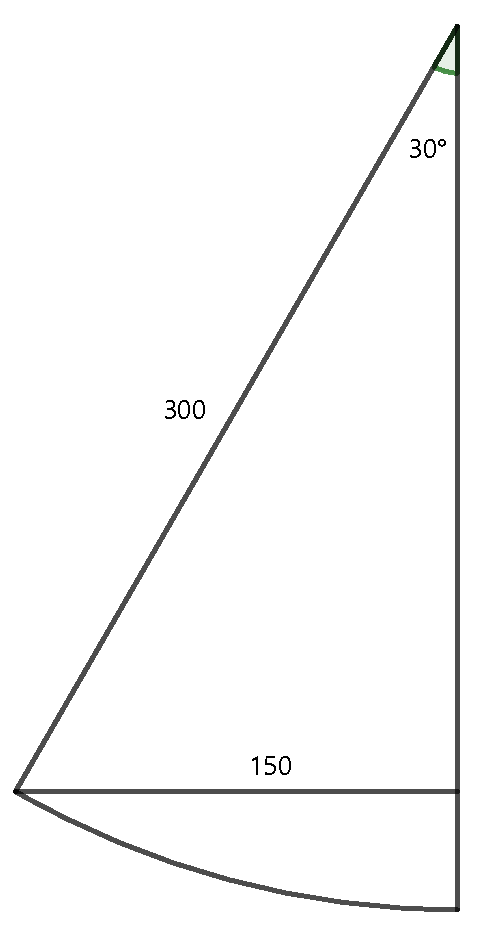
\includegraphics[height=0.2\textheight]{angle1.pdf}
    \end{minipage}
    \begin{minipage}[c]{0.48\textwidth}
        \centering
        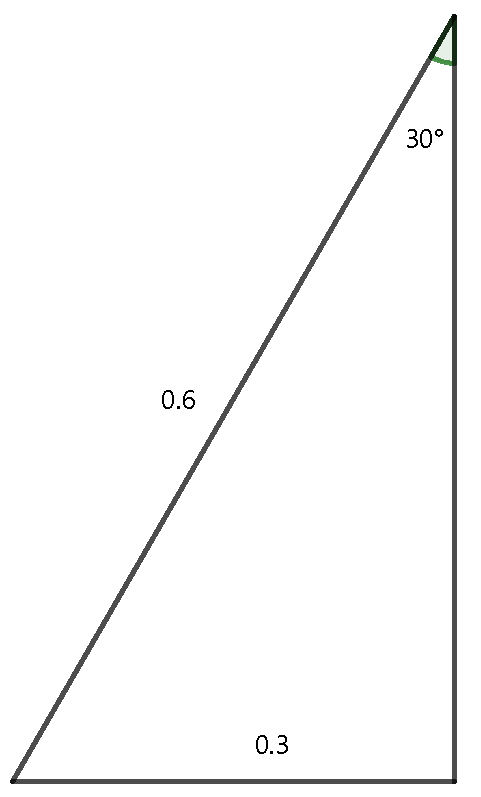
\includegraphics[height=0.2\textheight]{angle2.pdf}
    \end{minipage}
    \caption{}
    \label{fig:range}
\end{figure}

对于理想抛物面顶点的位置,本文采用蒙特卡洛法,对抛物面顶点进行打靶,搜索使由基准球面到工作态所有
筛选出的主索节点移动距离之和最小的抛物面顶点位置。

对于打靶范围的选择,由于促动器顶端径向伸缩量的范围是 $-0.6\sim +0.6m$。当抛物面顶点位置距离基准
球面过远时,绝大多数促动器所需调节的距离可能超过 $-0.6\sim +0.6m$。随着顶点由基准球面圆心向下移
动,调节距离之和呈现先减小后增大的趋势。在贴近基准球面处其值较小,故本文选择的范围为$\left[R-1.2,
R+1.2\right]m$。

若抛物面的顶点为 $(0,0,-a)$,可以通过焦点 $P$ 和顶点,进而确定抛物面的方程,记 $p$ 为焦距,
$p = a-R \times 0.534$,抛物面的公式为
\begin{equation}
    \label{eq:paraboloid}
    x^2 + y^2 = 4p(z + a)
\end{equation}
由于促动器伸缩沿基准球面径向,所以主索节点的位置移动均在一条
过基准球面球心的直线上,可以通过球心坐标 $(x_1,y_1,z_1)$ 和主索节点坐标 $(x_2,y_2,z_2)$ 计算得
这个直线的方程为
\begin{equation}
    \label{eq:line}
    \frac{\displaystyle x - x_1}{\displaystyle x_2 - x_1} = \frac{\displaystyle y - y_1}
    {\displaystyle y_2 - y_1} = \frac{\displaystyle z - z_1}{\displaystyle z_2 - z_1}
\end{equation}
联立方程 \eqref{eq:paraboloid} 与 \eqref{eq:line} 解得忽视促动器调节因素的情况下最理想的主索
节点坐标为
\[
\begin{dcases}
    \smallskip
    x = \frac{(2\times x_2\times (p\times z_2 + \sqrt{p\times (a\times x_2^2 + a\times
    y_2^2 + p\times z_2^2)}))}{(x_2^2 + y_2^2)}  \\
    \smallskip
    y = \frac{(2\times x_2\times (p\times z_2 + \sqrt{p\times (a\times x_2^2 + a\times
    y_2^2 + p\times z_2^2)}))}{(x_2^2 + y_2^2)(x_2 \times y_2)}  \\
    z = \frac{(2\times x_2\times (p\times z_2 + \sqrt{p\times (a\times x_2^2 + a\times
    y_2^2 + p\times z_2^2)}))}{(x_2^2 + y_2^2)(x_2 \times z_2)}  \\
\end{dcases}
\]

在此范围中以大
步长 $0.1$ 对抛物面顶点坐标进行枚举。并根据每次的枚举来调节相关主索节点的位置,使其位于或尽量贴
近理想抛物面。在调节完位置后,其中的一些主索节点很有可能已经超出了口径为 $300m$ 的工作抛物面,
我们需要对其再进行一次筛选,将那些超出工作抛物面范围的主索节点去除。可以通过坐标是否满足
$x^2 + y^2 \leqslant 150^2$ 来判断主索节点是否超出范围。



\subsubsection{模型的解}
在附件中,我们通过计算主索节点的坐标为,结合题目中给出球面半径约为 $300$,可以得到 $R = 300.4$。
在 $a$ 的取值范围内对 $a$ 进行枚举,得出最优值 $a = 299.90245$。
可算出 $p = 139.4888$,所以得到的理想抛物面的方程为
\[
    x^2 + y^2 = 562.3456(y + 300.9053)
\]
\subsection{问题二}
\subsubsection{模型的建立}
根据附件 $1$ 建立空间直角坐标系,该坐标系的
\subsubsection{模型的解}
\subsection{问题三}
\subsubsection{模型的建立}
\subsubsection{模型的解}
\nocite{宋叶志2019}
\bibliography{references}
\begin{appendices}
\section{第一问MATLAB代码一(大步长)}
\begin{lstlisting}[language=matlab]
clear all, clc;

%读入数据
data = xlsread("附件1.csv", 1, 'B2:D2227');%(n*3的矩阵)
data2 = [];
cnt2 = 0;
for i = 1:2226
    x = data(i,1);
    y = data(i,2);
    z = data(i,3);
    if x^2+y^2 <= 150.3^2
        data2 = [data2; i, x, y, z];
        cnt2 = cnt2 + 1;
    end
end
anss = inf;
finala = 0;
for a = 300.4-1.2:0.1:300.4+1.2
    s = 0;
    p = a-300.4*0.534;
    for i = 1:cnt2
        num = data2(i,1);
        x2 = data2(i,2);
        y2 = data2(i,3);
        z2 = data2(i,4);
        ansx1 = (2*x2*(p*z2 + sqrt(p*(a*x2^2 + a*y2^2 + p*z2^2))))/(x2^2 + y2^2); 
        ansy1 = ansx1 / x2 * y2;
        ansz1 = ansx1 / x2 * z2;
        ansx2 = (2*x2*(p*z2 - sqrt(p*(a*x2^2 + a*y2^2 + p*z2^2))))/(x2^2 + y2^2);
        ansy2 = ansx2 / x2 * y2;
        ansz2 = ansx2 / x2 * z2;
        if ansz2 < ansz1
            ansx = ansx2;
            ansy = ansy2;
            ansz = ansz2;
        else
            ansx = ansx1;
            ansy = ansy1;
            ansz = ansz1;
        end
        if ansx^2 + ansy^2 <= 150^2
            s = s + sqrt((ansx - x2)^2 + (ansy - y2)^2 + (ansz - z2)^2);
        end
    end
    if anss > s
        anss = s;
        finala = a;
    end
end
finala
\end{lstlisting}
\section{第一问MATLAB代码二(小步长)}
\begin{lstlisting}[language=matlab]
clear all, clc;

%读入数据
data = xlsread("附件1.csv", 1, 'B2:D2227');%(n*3的矩阵)
data2 = [];
cnt2 = 0;
for i = 1:2226
    x = data(i,1);
    y = data(i,2);
    z = data(i,3);
    if x^2+y^2 <= 150.3^2
        data2 = [data2; i, x, y, z];
        cnt2 = cnt2 + 1;
    end
end
anss = inf;
finala = 0;
for a = 299:0.00001:301
    s = 0;
    p = a-300.4*0.534;
    for i = 1:cnt2
        num = data2(i,1);
        x2 = data2(i,2);
        y2 = data2(i,3);
        z2 = data2(i,4);
        ansx1 = (2*x2*(p*z2 + sqrt(p*(a*x2^2 + a*y2^2 + p*z2^2))))/(x2^2 + y2^2); 
        ansy1 = ansx1 / x2 * y2;
        ansz1 = ansx1 / x2 * z2;
        ansx2 = (2*x2*(p*z2 - sqrt(p*(a*x2^2 + a*y2^2 + p*z2^2))))/(x2^2 + y2^2);
        ansy2 = ansx2 / x2 * y2;
        ansz2 = ansx2 / x2 * z2;
        if ansz2 < ansz1
            ansx = ansx2;
            ansy = ansy2;
            ansz = ansz2;
        else
            ansx = ansx1;
            ansy = ansy1;
            ansz = ansz1;
        end
        if ansx^2 + ansy^2 <= 150^2
            tmps = sqrt((ansx - x2)^2 + (ansy - y2)^2 + (ansz - z2)^2);
            if tmps > 0.6
                tmps = 0.6;
            end
            s = s + tmps;
        end
    end
    if anss > s
        anss = s;
        finala = a;
    end
end
finala
\end{lstlisting}
\section{第二问MATLAB代码}
\begin{lstlisting}[language=matlab]
\end{lstlisting}
\section{第三问MATLAB代码}
\begin{lstlisting}[language=matlab]
\end{lstlisting}
\end{appendices}
\end{document}